\section{Theorie}
\label{sec:Theorie}

Bevor konkret auf das Spektrum von Gammastrahlern und die Funktionsweise von Germaniumdetektoren eingegangen wird, sollen zunächst einige zum
Verständnis wichtige Grundlagen wiederholt werden.

\subsection{Gammastrahlung}

\begin{figure}
    \centering
    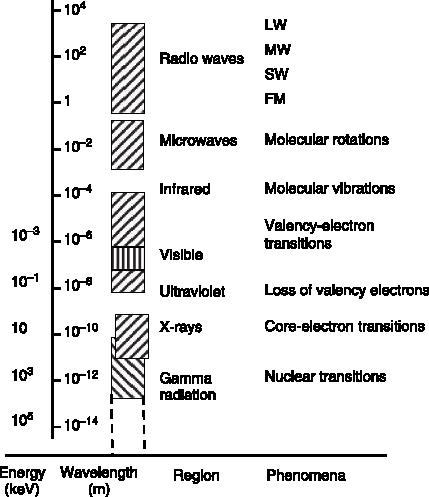
\includegraphics{figures/light_energies.pdf}
    \caption{Grafische Darstellung des elektromagnetischen Spektrums zu unterschiedlichen Wellenlängen \cite{gamma}.}
    \label{fig:ems}
\end{figure}

Als Gammastrahlung werden Photonen, also elektromagnetische Strahlung, mit einer Energie zwischen circa $\SI{10}{\kilo\eV}$ und $\SI{10000}{\kilo\eV}$ bezeichnet.
Anders als bei $\alpha$- und $\beta$-Strahlung handelt es sich bei $\gamma$-Strahlung um ungeladene Strahlung mit hoher Reichweite und Eindringtiefe.
Gammastrahlung kann durch unterschiedliche Prozesse, darunter z.B. der Zerfall von Positronen und anderen Teilchen oder Bremsstrahlung entstehen.
Da hier aber das Gammaspektrum von Atomkernen betrachtet werden soll, sind insbesondere Photonen, die in Kernzerfällen entstehen, wichtig.
Findet in einem Kern ein $\alpha$- oder $\beta$-Zerfall statt, verbleibt der Kern oft in einem angeregten und instabilen Energiezustand.
Dort fällt er nach einer bestimmten Zeit (meistens in der Größenordnung einiger $10^{-12}\, \si{\second}$) in einen stabilen niederenergetischen Zustand zurück.
Die Energiedifferenz zwischen den beiden Zuständen wird in Form eines Photons abgestrahlt \cite{gamma}. \\

Diese Photonen verlassen den Kern und können auf verschiedene Weise mit der umliegenden Materie interagieren.

\subsubsection{Photoeffekt}

Beim Photoeffekt wird das emittierte Photon von einem Elektron absorbiert.
Ist die Photonenenergie höher als die Bindungsenergie $E_\text{B}$, die das Elektron an den Kern bindet, wird es mit der Energie $E_\text{e} = E_\gamma - E_\text{B}$
aus der Atomhülle emittiert.
Das freie Elektron gibt seine Energie durch die Emission weiterer Photonen oder Kollisionen mit anderen Elektronen ab.
Da das Photon vollständig absorbiert wird kann dieser Prozess zur Energiebestimmung genutzt werden.

\subsubsection{Comptoneffekt}

Anders als beim Photoeffekt beschreibt der Comptoneffekt, auch Comptonstreuung, wie in \autoref{fig:comptonscattering} die Streuung eines Photons an einem Elektron.

\begin{figure}
    \centering
    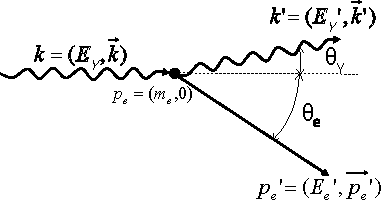
\includegraphics{figures/compton.pdf}
    \caption{Schematische Darstellung der Streuung eines Photons an einem Elektron \cite{Teilchendetektoren}.}
    \label{fig:comptonscattering}
\end{figure}

Bei der Streuung wird abhängig vom Streuwinkel ein Energiebruchteil
\begin{equation}
    E_{\gamma'} = E_\gamma \frac{1}{1 + \varepsilon (1 - \cos\theta)}
    \label{eq:Egammaprime}
\end{equation}
an das Elektron übertragen. \\
Mit $\varepsilon = \frac{E_\gamma}{m_\text{e} c^2}$ ist die Elektronenenergie nach der Streuung durch
\begin{equation}
    E_\text{e} = E_\gamma -E_{\gamma'} = E_\gamma (1 - \frac{1}{1 + \varepsilon (1 - \cos\theta)}) 
\end{equation}
gegeben. \\

Die Klein-Nishima-Gleichung liefert dann den differentiellen Wirkungsquerschnitt
\begin{equation}
    \frac{\text{d}\sigma_C}{\text{d}\Omega} = \frac{r_\text{e}^2}{2 (1 + \varepsilon (1 - \cos\theta))^2} 
                                              \left(1 + \cos^2\theta + \frac{\varepsilon^2 (1 - \cos\theta)^2}{1 + \varepsilon (1 - \cos\theta)} \right)
                                              \label{eq:dcrossomega}
\end{equation}
pro Raumwinkel und freiem Elektron, der sich mit $t = \frac{E_\text{e}}{E_\gamma}$ auch als Ableitung nach der Elektronenenergie darstellen lässt, sodass
\begin{equation}
    \frac{\text{d}\sigma_C}{\text{d}E_\text{e}} = \frac{\pi r^2_\text{e}}{m_\text{e} c^2 \varepsilon^2} 
                                                  \left(2 + \frac{t^2}{\varepsilon^2 (1-t)^2} + \frac{t}{1-t} \left(t - \frac{2}{\varepsilon}\right)\right)
    \label{dcrossE_e}
\end{equation}
ebenfalls den differentiellen Wirkungsquerschnitt beschreibt \cite{Teilchendetektoren}.

\subsubsection{Paarerzeugung}

Da der hier verwendete Detektor eine obere Energieschranke von etwa $\SI{5}{\mega\eV}$ aufweist ist die Paarerzeugung der höchstenergetische relevante Prozess.
Im Coulombfeld eines Atomkerns produziert das Photon ein $e^+ e^-$-Paar, von denen das Positron in den meisten Fällen in kurzer Zeit mit einem Hüllenelektron annihiliert,
sodass das Elektron detektiert werden kann.
Da hier ein Paar mit einer Ruhemasse von etwa $\SI{1000}{\kilo\eV}$ erzeugt wird ist auch die Energiegrenze dieses Prozesses ähnlich hoch.



